% !TeX encoding = UTF-8
%% (requires IEEEtran.cls version 1.7 or later) with an IEEE conference paper.
\documentclass[journal]{IEEEtran}

\renewcommand\IEEEkeywordsname{Keywords}

\pagenumbering{gobble}

\usepackage[utf8]{inputenc}

% *** GRAPHICS RELATED PACKAGES ***
%\usepackage[pdftex]{graphicx}
\usepackage{graphicx}
%\usepackage[dvips]{graphicx}
% to place figures on a fixed position
\usepackage{float}


% *** PDF, URL AND HYPERLINK PACKAGES ***
\usepackage{url}

% correct bad hyphenation here
\hyphenation{NetFPGA}

\usepackage{xcolor}

\usepackage{siunitx}

\usepackage{bytefield}

\usepackage{amsmath}
\usepackage{amssymb}
\usepackage{algorithm}
\usepackage{algorithmic}

% \renewcommand\note[1]{} % uncomment this line to hide notes

%%%%%%%%%%%%%%%%%%%%%%%%%%%%%%%%%%%%%%%%%%%%%%%%%%%
%%%%%%%%%%%%%%%%%%%%%%%%%%%%%%%%%%%%%%%%%%%%%%%%%%%
%%%%%%%%%%%%%%%%%%%%%%%%%%%%%%%%%%%%%%%%%%%%%%%%%%%
%


% LaTeX quick ref
%
% \cite{refname} to place citation
%
% \label{label_name} to place a label, which can be reference by \ref{label_name}
%
% new paragraph -> empty line between text
%
% \noindent to not indent paragraphs first line
%
% create list with : \begin{itemize} \end{itemize}
% \begin{itemize
% \renewcommand to renew numbering \labelitemi{--} to select bullet type
% \item item elem 1
% \item item elem2
% \end{itemize}
%
% et alia (et al.) should be emphasized (i.e in italic) with \emph{et al.}
%
% to add figure, htb is placement selector , !overrid internal paramters
%\begin{figure}[!htb]
%    \centering
%    \includegraphics[width=0.5\textwidth]{FIG.png}
%    \caption{Caption}
%    \label{fig:label}
%\end{figure}
%
% ~ concatenates dynamic text with literals
%
% long dash is --
%
% `is single quoted' , ``is double qouted"
%
% to autoformat with latexindent: latexindent -w  -m -l defaultSettings.yaml ProtoImplFPGA.tex


\begin{document}
% conference papers do not typically use \thanks and this command
% is locked out in conference mode. If really needed, such as for
% the acknowledgment of grants, issue a \IEEEoverridecommandlockouts
% after \documentclass
% paper title
% can use linebreaks \\ within to get better formatting as desired
\title{Time Synchronization Solution for FPGA-based Distributed Network Monitoring}
%\titleheader{25th Telecommunications forum TELFOR 2017 \hfill Serbia, Belgrade, November 21-22, 2017.}

% author names and affiliations
% use a multiple column layout for up to three different
% affiliations
\author{Ferenc Nandor Janky and Pal Varga \thanks{The authors are with the Department of Telecommunications and
 \mbox{MediaInformatics}, Faculty of Electrical Engineering and Informatics,
Budapest University of Technology and Economics,
Magyar tudósok körútja 2., 1117 Budapest, Hungary (phone: +36704213213; e-mail: \mbox{fecjanky@gmail.com} and pvarga@tmit.bme.hu)}}
%\IEEEauthorblockN{Ferenc N\'{a}ndor Janky and P\'{a}l Varga}
%\IEEEauthorblockA{Dept. of Telecommunications and Media Informatics\\Budapest University of Technology and Economics\\
%2 Magyar Tud\'{o}sok krt., Budapest, Hungary, H-1117\\
%Email: \{fjanky, pvarga\}@tmit.bme.hu }

%
%}%


% make the title area
\maketitle

\begin{abstract}
    \boldmath
    Distributed network monitoring solutions face various challenges with the increase of line speed, the extending variety of protocols, and new services with complex KPIs. This paper addresses one part of the first challenge: faster line speed necessitates time-stamping with higher granularity and higher precision than ever. Proper, system-wide time-stamping is inevitable for network monitoring and traffic analysis point of view. It is hard to find feasible time synchronization solutions for those systems that has nation-wide, physically distributed probes.
    
    Current networking equipment reside in server rooms, and have many legacy nodes. Access to GPS signals are complicated in these places, and Precision Time Protocol (PTP) is not seem to be supported by all network nodes in the near future -- so high precision time-stamping is indeed a current problem. This paper suggests a novel, practical solution to overcome the obstacles. 
    
    The core idea is that in real-life, distributed network monitoring systems operate with a few, finite number of probe-clusters, and their site should have a precise clock provided by PTP or GPS somewhere in the building. The distribution of time information within a site is still troublesome, even within a server rack. This paper presents a closed control loop solution implemented in an FPGA-based device in order to minimize the jitter, and compensate the calculated delay.
    
\end{abstract}

\begin{IEEEkeywords}
    network monitoring, time synchronization, hardware acceleration, closed control loop 
\end{IEEEkeywords}

% no keywords
\section{Introduction}\label{sec:Intro}

Network monitoring has a well-established practice at telecommunication operators. There are fundamentally different solutions available -- depending on what kind of data are initially available and how it is gathered. The least flexible solutions are based on the functional networking elements: they can provide pre-digested reports, statistical counters, and occasionally (when not under heavy load), even detailed information on the actual messages. Some operators use standalone protocol analyzers, which do not suffer from the temporal, load-related bottlenecks -- rather, they have spatial data capture issues: only a segment of the network is visible at any given time. On the other hand, complete traffic information can be gathered by network-wide traffic monitoring. These latter solutions are based on passive, distributed probes; central processing entities; and client software -- also distributed -- at the operating personnel. This paper discusses a peculiar problem of such systems: effective time synchronization among the entities.

Network traffic analysis requires the understanding of the order of the messages appearing in the network, even if they appear at different interfaces. This makes high resolution and high precision timestamping the basic requirement, beside lossless message capture. 
While there are standardized network protocols available for tackling this issue, there are practical obstacles in their network-wide usage. Although the Network Time Protocol (NTP) is widely available \cite{NTP_book}, it cannot be used as a general purpose synchronization protocol. In fact, the message transfer delay between NTP clients and servers are not compensated, hence the different nodes end up setting their local time to a clock value with a random delay. The typical order of the forwarding delay in current core routers is in the 0.5-5 microseconds range, depending on the traffic volume -- among other factors. Since the minimum packet interarrival-time is 0.672 microsecond even at a 1Gbit\/s link (and 67.2 nanoseconds for a 10Gbit\/s link), such delays cannot be left without compensation for time synchronization.

Precision Time Protocol (PTP), on the other hand covers the delay-compensation issue well \cite{PTP_standard}. Unfortunately, PTP is not at all wide-spread, even after 10 years of commercialization for PTPv2. The concept, however, necessitates that all network nodes in the path have PTPv2 capability. Otherwise -- even if one node cannot compute and share its delay data --, compensation of time information is not possible.

Another solution could be to introduce time information of GPS (Global Positioning System) satellites into the nodes -- this is not feasible, since rack cabinets in server rooms lack the line of sight.

We can suppose that at least one machine at each monitoring site has the possibility to get synchronized to the master clock of the network (e.g. through PTP or GPS). Nevertheless, synchronizing all clocks within the site with nanosecond-range precision, is still a challenge.

This paper presents a solution for the time synchronization issues of systems with FPGA-based monitoring probes. What makes FPGA a key player here is that hardware-acceleration removes the jitter of operating system and protocol-stack delay from the equation. The delay of handling time information within an FPGA is constant, we can calculate with it precisely -- and compensate this delay for the time-stamp.

In this paper we focus of the time synchronization challenges of a monitoring site. The implemented solution is based on the practical pre-requisite that each site has a reference clock available for the monitoring system. This paper suggests an FPGA-based clock synchronization method for the distributed monitoring equipment, more precisely, its interface cards.

\begin{figure*}[!htb]
    \centering
    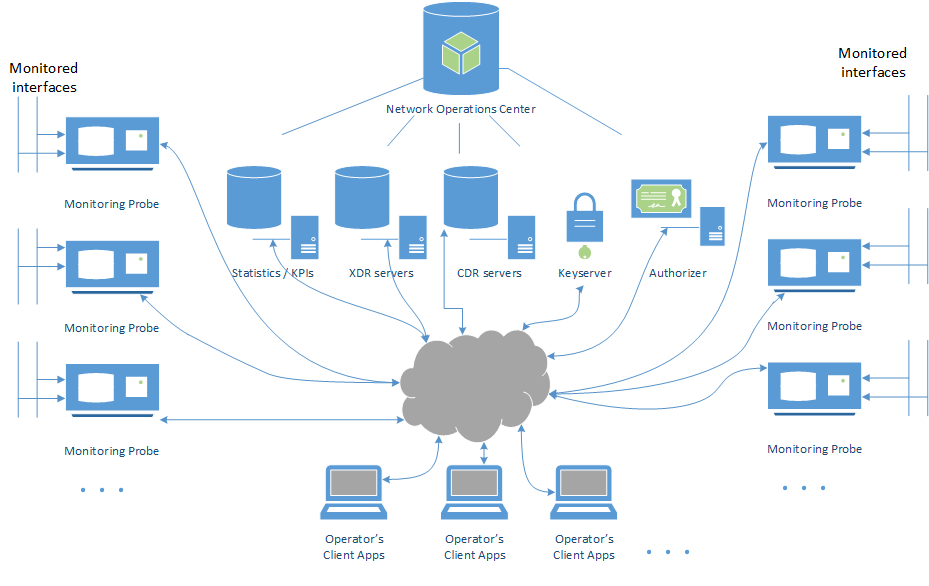
\includegraphics[width=0.9\textwidth]{figures_raw/Network_monitoring.png}
    \caption{A generic architecture for distributed network monitoring}
    \label{fig:network_monitoring}
\end{figure*}

\section{Network Monitoring supported by FPGA-based Probes}\label{sec:NetMon}
\subsection{The Generic Concept of Distributed Network Monitoring}

The distributed network monitoring architecture depicted by Figure~\ref{fig:network_monitoring} supports local, probe-based pre-processing (timestamping, requirement-based packet chunking, filtering criteria-based distribution) and central, deep analysis (correlation of messages and transactions, data record compilation, statistics generation), even on-the-fly. The time-based ordering and interleaving of messages are enabled by the hardware-accelerated timestamping, providing nanosecond-range resolution with sub-microsecond precision. The information stored locally at the distributed Monitoring Probes can be accessed by client applications of the operator. Besides, the Monitoring Probes send pre-digested data to the Servers for correlation (creating e.g. Call Data Records, CDRs), as well as periodic reports containing their calculated statistics \cite{Tatai_mobile_analysis}.

Since user data and control data are often carried over the same channels, their division requires message analysis on network- or transaction-level (e.g., IP- or TCP-level). The changing traffic patterns force the operators to look for new tools to process even the user traffic. The first step towards this is the compilation of XDRs (eXtended Data Records) based on control- and user-plane messages and transactions. These often contain message-level timestamps, as well. Based on these data, the deep traffic analysis tools provide valuable information towards business-intelligence and network optimization. Besides, all nodes can be configured to report directly to the NOC (Network Operations Center).

Operators use the network-wide, passive monitoring for fault detection, service quality assurance, and resource planning, among others \cite{LTE_monitoring}. Besides lossless data capture, network monitoring covers further functions, as well:
\begin{itemize}
\renewcommand\labelitemi{--}
\item precise timestamping, ordering;
\item compilation, search and fetch of Call Data Records (CDRs) and Extended Data Records (XDRs);
\item calculation and reporting of Key Performance Indicators, KPIs;
\item Call Tracing at various complexity levels;
\item bit-wise message decoding for protocol analysis; etc. 
\end{itemize}

All these functions are present in the network monitoring practice, since beside user-level data analysis, network analysis is important from connection-level to application-level, as well.

System elements of the described generic architecture can be implemented in many ways. In the SGA-7N system -- which serves as the base implementation for the presented solution --  monitoring probes of the presented system are called ``Monitors''. These consist of three main building blocks: a high performance Field Programmable Gate Array (FPGA)-based custom hardware platform, a firmware dedicated for network monitoring, and the probe software \cite{AITIA_SGA7N}.

\subsection{FPGA-based packet processing}

There are many features that make FPGAs useful in packet processing tasks \cite{NetFPGA}. The main concept itself allows \emph{parallel processing} of the input data. Different, simultaneous tasks can be carried out at each clock cycle on the same data, which in this case is the packet header \cite{XILINX_PacketProc}, \cite{Weirong_Scalable_PacketProc_FPGA}. Besides, the \emph{input word length} is much greater for FPGAs (getting 90 bytes) than for modern CPUs (64 bits). Furthermore, FPGA are set up in hardware-defined languages, and they are indeed \emph{reconfigurable} hardware: their internal wiring can be changed within milliseconds. These features enable FPGA-based hardware platforms to become high performance networking devices, e.g., network monitors, switches, routers, firewalls or intrusion detection systems \cite{IM_2015_FPGA}. Nevertheless, as a network monitoring system, it supports distributed and lossless packet level monitoring of Ethernet links for 1 or 10 Gbit\/s.

Beside providing sufficient resources for switching and routing at 1 or 10 Gbit\/s, the design of SGA-GPLANAR \cite{GPLANAR} and SGA-10GED \cite{10GED} used in SGA-7N includes some special, network monitoring-related requirements, namely 
\begin{itemize}
\renewcommand\labelitemi{--}
\item lossless packet capture,
\item 64-bit timestamping with sub-microsecond resolution,
\item header-only capture: configurable depth of decoding,
\item on-the-fly packet parsing by hardware \cite{Low_Latency_Header_Parser},
\item parameterized packet/flow generator for mass testing \cite{Olaszi_Complex_Load_Testing_of_Mobile_PS_and_CS_Core},\cite{Soos_Mesterproba}.
\end{itemize}

Various applications then require other supported functionalities. As an example, the high-speed monitoring application \cite{C-GEP_HPSR} consists of the following sub-modules:
\begin{itemize}
\renewcommand\labelitemi{--}
\item timestamping every frame upon reception;
\item packet decoding from layer 2  up to the application layer;
\item packet filtering with a reconfigurable rule-set to decide what we do with a given packet;
\item packet chunking: packets can be truncated depending on the matching rule;
\item packet distribution: to distribute packets by different criteria: IP flows, fragment steering, steering based on mobile core network parameters, etc.;
\item packet headering: monitoring information is stored in a specified header format.
\end{itemize}

These features and capabilities make the FPGA a suitable enabler of hardware acceleration within the Monitors.

\section{Challenges and Requirements in Detail}\label{sec:Challanges}

%TODO(Fec) : 0.5 oldal
%- Monotonic clock
%- Remote locations, skewing clock
%- Adaptation to legacy systems 
%- Precision requirements (Fendler Tomi TDK)

For a distributed monitoring solution described in the previous sections, there is a strong requirement for having
a \emph{monotonic clock}. Otherwise, packet reordering would happen even with a single monitoring node (changing its clock) -- and this is not feasible, since traffic analysis is heavily dependent upon packet timestamps. As a consequence, the need for monotonic system time is inherent.

Another challenge comes from the fact that a distributed monitoring system has its components geographically
separated from each other, therefore the clock frequency and the time information of the clocks of the nodes have to be
frequency- and phase-synchronized to each other with some given threshold. This problem has many solutions, e.g., using
GPS based synchronization
systems~\cite{GPS-CLOCK}. Although technically it can work well \cite{NetFPGA_GPS}, as a drawback, this requires additional installation expenditures on an indoor site that has no installed
antenna system to carry the GPS signal inside the building and could also result in extensive cabling work. 
A convenient alternative is to use network time synchronization that utilizes the telecommunication network for
exchanging packets as per a designated protocol to achieve frequency and phase synchronization. Examples for this
are Network Time Protocol (NTP)~\cite{NTP_book} and Precision Time Protocol (PTP)~\cite{PTP_standard}.

When speaking about time synchronization, the following properties describe a clock -- which are in-line with the generic definition of clock properties \cite{NTP_IEEEToN}:
\begin{itemize}
    \item accuracy -- \emph{i.e.} how good is the time information compared to some reference
    \item precision -- \emph{i.e.} how precise is a tick of the clock compared to some reference
    \item stability -- \emph{i.e.} how does the clock frequency change	e.g., over time or based on external
          temperature changes etc.
\end{itemize}

The biggest challenge of all -- as usual -- is to adapt to the existing monitoring framework described in
\ref{sec:NetMon}
with minimal modifications to the existing solution, while satisfying all the precision and accuracy related requirements.
As mentioned before, the platform for proof-of-concept is the SGA-7N monitoring system, which utilizes FPGA-based monitoring cards. These are capable of capturing on high-speed network interfaces -- with fine-grained timestamping capabilities --, and they have their own, existing time-keeping facilities.

In order to tackle all the above mentioned issues with a solution fitting into the network monitoring architecture, we suggested to create a new FPGA-based card that implements these functions:
\begin{itemize}
    \item network time synchronization,
    \item local time synchronization,
    \item interfacing with the existing nodes -- OAMP functions.
\end{itemize}

The following sections describe this solution, and show its feasibility in the running monitoring system.

\IEEEpubidadjcol %%%%%% ezmiez? %%%%%%%%%%

\section{Architecture of the Distributed Time Synchronized Monitoring System}

\subsection{Generic concept}
For providing easy adaptation into the existing system, and also taking into account FPGA resource usage, a hybrid
solution
has been designed. This solution implements network time synchronization in a standalone card that distributes the digital timing
information over a dedicated control bus, as illustrated by Figure~\ref{fig:concept}.

The synchronization framework provides a platform-independent agent that
can be integrated into the existing FPGA cards' top level VHDL (VHSIC Hardware Description Language, \cite{VHDL_standard}) modules, and is used through a well-defined and portable interface.

The agent itself has low complexity, and as a result, the solution does not waste CLB (Configurable Logic Block) resources -- as if the whole network
synchronization stack were instantiated N times on all monitoring node cards. Furthermore, this results in better internal
synchronization
compared to the replicated stacks, since those can have skew to each other (within the boundaries), as specified by their
protocol.

\begin{figure}[!htb]
    \centering
    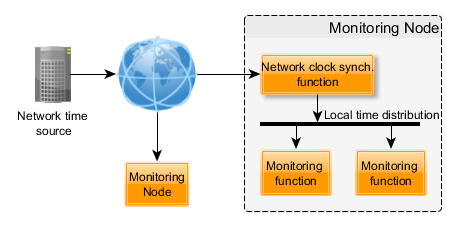
\includegraphics[width=0.45\textwidth]{figures_raw/concept.png}
    \caption{Fitting the time synchronization function into the generic, distributed network monitoring concept}
    \label{fig:concept}
\end{figure}

As shown by Figure~\ref{fig:concept}, each node has its own network synchronization function, therefore the accuracy and
precision between two monitoring nodes can be guaranteed only to an extent that the utilized time synchronization
protocol provides. Due to the uncompensated delay of routers, switches and transmission paths, this is in the magnitude of milliseconds of a software implementation of NTP. This precision, can be increased by using FPGAs for hardware acceleration. Depending on the PTP version and the underlying network capabilities, this can fall into the magnitude of nanoseconds.

The main idea of the solution is to install a local time-distribution bus between the nodes within a site. This allows us to achieve nanosecond-range synchronicity, as there is
less perturbation between the hardware implementations of the transmitting and receiving ends -- no OS scheduler, no network etc. Moreover, frequency synchronization can also be easily achieved by implementing a synchronous bus -- i.e., transmitting
the
clock signal along with the data.

\subsection{External time synch. subsystem design and implementation}\label{sec:External-Impl}

When selecting the candidate for implementing the external time synchronization function, three protocols were considered:
\begin{itemize}
    \item Network Time Protocol (NTP) \cite{NTP_book},
    \item Precision Time Protocol v1 (PTPv1) \cite{PTPv1},
    \item Precision Time Protocol v2 (PTPv2) \cite{PTP_standard}.
\end{itemize}

In order to achieve the best synchronization between PTPv2 clocks, the protocol requires PTPv2-enabled switches/routers throughout the network. These do the bookkeeping of the processing delay values in the synchronization packets as they traverse through the network. Without this feature, the achievable synchronicity in a multi-hop network is around the same as by using PTPv1.

Since PTPv2 is not widely available in current networks, we concluded in either selecting NTP or PTPv1, due to their simplicity. PTPv1 has way more modes of operation when compared to NTP. Still, these two protocols are operating based on semantically the same principle when determining the round
trip time and offset
compared to a reference clock entity. Although there are significant differences originated from their packet structure, the
timestamp format and also the epoch that could result in more complex implementation if PTPv1 would be chosen.
Still, the NTP timestamp format includes a 32-bit unsigned seconds field spanning 136 years and a 32-bit fraction field resolving 232
picoseconds the prime epoch, or base date of era 0, is 0 h 1 January 1900 UTC -- i.e., when all bits are zero.

Based on the requirements, the above considerations, and the Occam principle, the design decision led to selecting \emph{NTP protocol to be used} for synchronizing the
FPGA-based monitoring cards through a card that is responsible for implementing the external and internal (see
Section~\ref{sec:Internal-Impl}) time synchronized function called SGA-Clock.

Each FPGA-based packet processing and networking protocol implementation has its own complexity. There are several
readily available implementations that can be used for packet processing in FPGAs with some limited flexibility when it
comes to interconnecting it
with other modules. The one that has been used for the current implementation is a flexible solution for Protocol
Implementations within FPGAs. The solution detailed in \cite{ProtoImpl} provides a generic framework in VHSIC Hardware
Description Language (VHDL) that enables rapid prototyping of networking protocols. Among many other things it provides
the following main features:
\begin{itemize}
    \renewcommand \labelitemi{--}
    \item supports protocol module interconnection via layering;
    \item handles reception and transmission of Protocol Data Units (PDUs) with queuing;
    \item provides a high level interface for separating and combining	Protocol Control Information (PCI) and Service Data Unite (SDU),
          forwarding, pausing or dropping SDUs;
    \item provides a unified way to handle Interface Control Information (ICI), SDU, and PDU events (e.g., error signalling) \cite{ISO:OSI};
    \item adds support of auxiliary information that travels along with messages
    \item provides components for common tasks recurring during implementing networking protocols
          (de/serialization, arbitration etc.).
\end{itemize}

\begin{figure}[!htb]
    \centering
    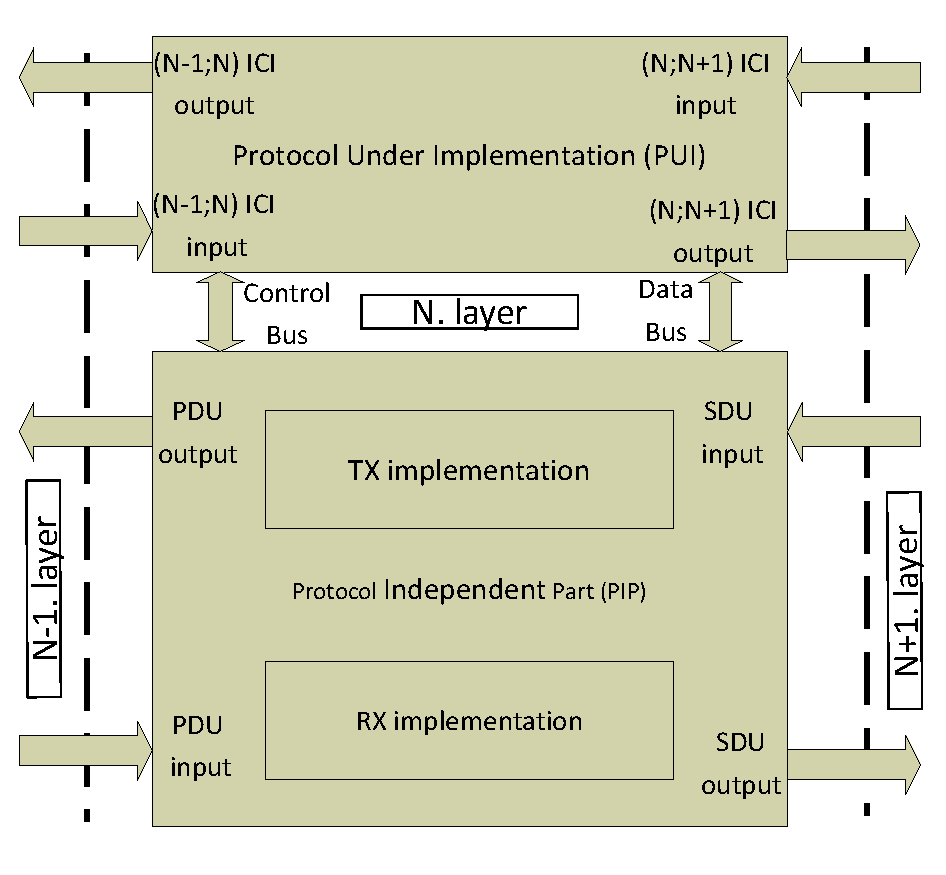
\includegraphics[width=0.4\textwidth]{figures_raw/system_sketch.pdf}
    \caption{Fundamental building block of the FPGA networking framework used for the Protocol Implementation}
    \label{fig:system_sketch}
\end{figure}

The framework's basic building block (shown by Figure~\ref{fig:system_sketch}) was used for implementing a pure FPGA-based
UDP/IP protocol stack with ARP \cite{ARP_RFC826} on top of 802.3 Ethernet. It provides a platform with deterministic timing for the
likewise FPGA-based
implementation of NTP. For each of these protocols the corresponding protocol-specific parts have been described in
VHDL, using the generic framework \cite{ProtoImpl}.

\begin{figure}[!htb]
    \centering
    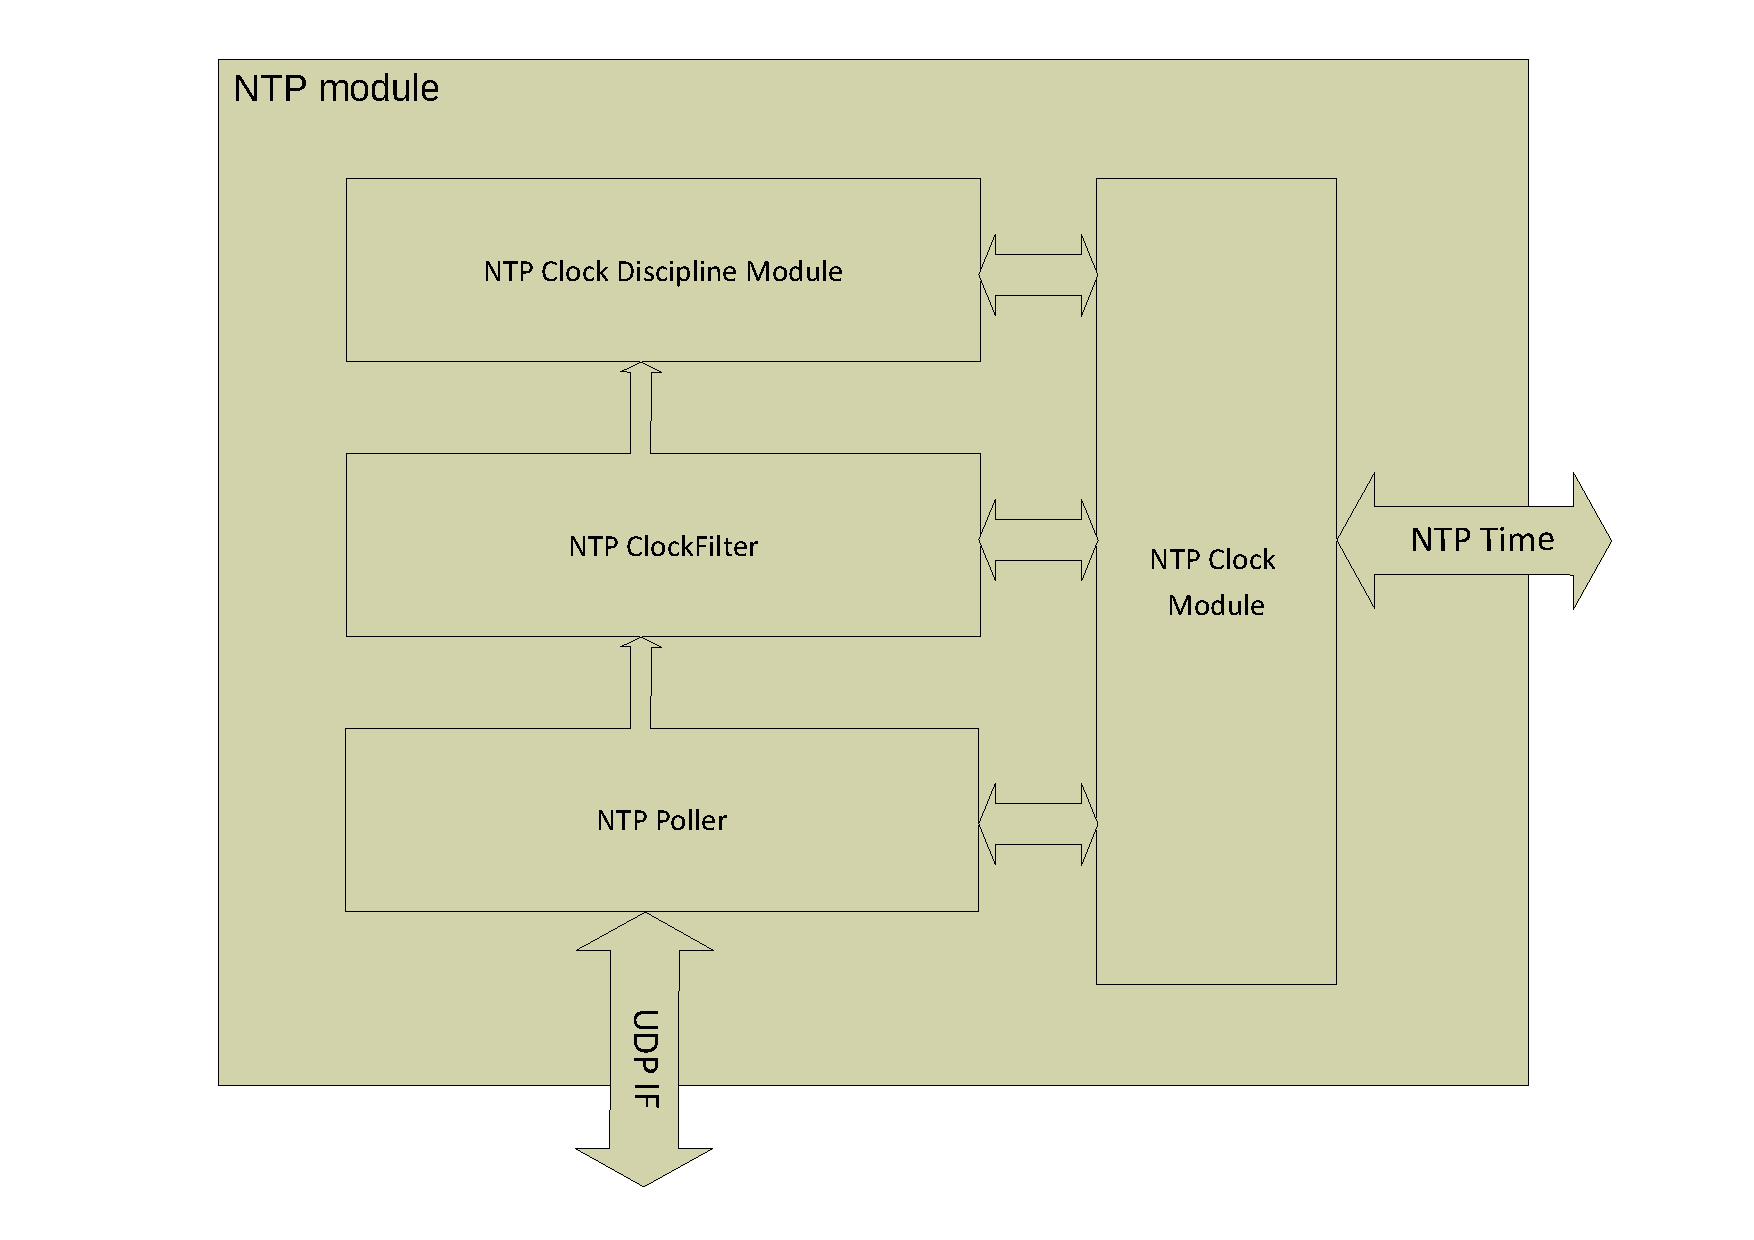
\includegraphics[width=0.5\textwidth]{figures_raw/ntp-sketch.pdf}
    \caption{NTP module block diagram of components}
    \label{fig:ntp-impl}
\end{figure}

The internal structure of the NTP module is shown by Figure~\ref{fig:ntp-impl}. The NTP Poller component is responsible
for the NTP packet transmission and reception, and implementing the On-Wire protocol
for determining the offset -- based on the packet messages. The packet-handling part is also implemented
through the Protocol Implementations framework. The NTP ClockFilter component is there to regulate the offset values
presented by the poller by ordering the results based on delay, updating internal state variables, calculating jitter,
and
suppressing spikes based on jitter and last successful test time. If the offset data got passed the filter stage, it gets
forwarded for further processing by the NTP Discipline module.

The NTP Discipline module controls the clock module -- by adjusting the time increment -- based on the filtered offset
data. The NTP clock module provides an interface for controlling the time increment that itself is added to the clock
register in each system clock cycle -- thus
implementing the clock functionality. The time information is fed back to each module as illustrated on
Figure~\ref{fig:ntp-impl}.
This chain of modules with the feedback is another realization of a closed loop control chain described in the following section.

\subsection{Internal time synch. subsystem design and implementation}\label{sec:Internal-Impl}

\begin{figure}[!htb]
    \centering
    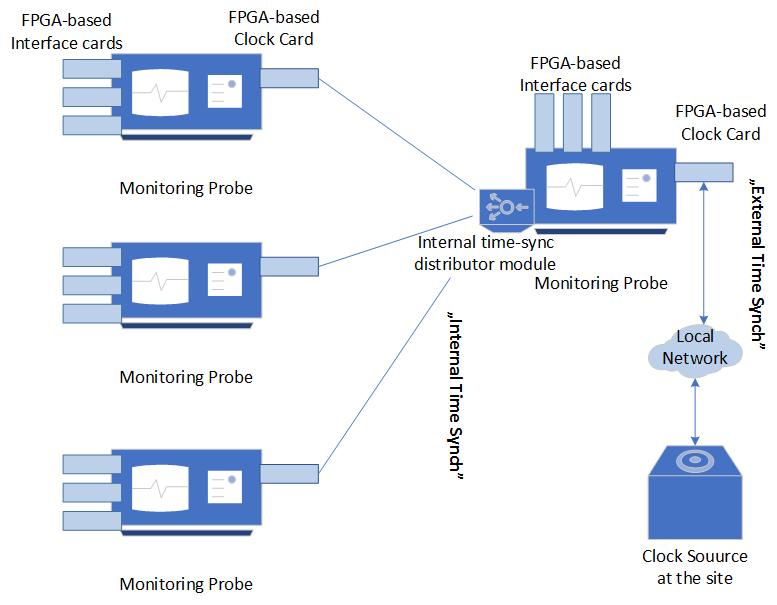
\includegraphics[width=0.5\textwidth]{figures_raw/TimeSynch_distribution.png}
    \caption{Time synchronization within a monitoring site -- methods for external and internal subsystems differ to allow high precision and accuracy in timestamping}
    \label{fig:TymeSinchArch}
\end{figure}

Since timestamping is done by the monitoring interface cards, the time synchronization information has to be spread around all interface cards of all monitoring units within the site. This time synchronization is an internal matter of the monitoring system. The relationship between ``external'' and ``internal'' time synchronization is shown by Figure~\ref{fig:TymeSinchArch}.

The internal time information synchronization function is responsible for having all clocks in all monitoring functions
to be completely synchronized \emph{within a monitoring node}. Since this is an internal component, the amount of perturbation
that potentially affects this subsystem is considered minimal compared to the external time synchronization subsystem.

The elements of this subsystem are:
\begin{itemize}
    \item digital bus that is able to transmit time and status information;
    \item a driver module of that bus that resides in the Network clock synchronization function;
    \item receiver modules attached to that bus performing local time synchronization.
\end{itemize}

Internally to each monitoring probe, all FPGA boards that implement a monitoring function can operate from different power supply units. As a
consequence, ground level
isolation is necessary over the bus. For reducing the physical layer complexity,
a point-to-point bus system has been designed. In order to be able to maximize the number of clients connected the
bus, it utilizes an asynchronous serial communication using 2 wires. The communication protocol executed by the driver
module (the internal time synch distribution module in Figure~\ref{fig:TymeSinchArch})
multiplexes arbitrary data units and the time information over the bus into frames -- equipped with error detection
code --
in an alternating pattern. That results in periodic transmission of valid time information.

The parameters of the physical signalling are:
\begin{itemize}
    \item LVCMOS33 (Low Voltage CMOS 3.3) levels for representing logical values;
    \item asymmetric signal transmission;
    \item \SI{15.625}{\mega\hertz} clock frequency with 4x oversampling;
    \item NRZ line coding.
\end{itemize}

\begin{figure}
    \begin{bytefield}{32}
        \bitheader{0-31} \\
        \bitbox{16}{All ones} & \bitbox{1}{S} & \bitbox{1}{T} & \bitbox{14}{time/data} \\
        & \wordbox{1}{time/data} \\
        & \bitbox{18}{time/data} & \bitbox{8}{CRC-8}
    \end{bytefield}
    \caption{High-Speed Timestamp Interface frame format}
    \label{fig:HiSTI-frame}
\end{figure}

\begin{figure*}[!htb]
    \centering
    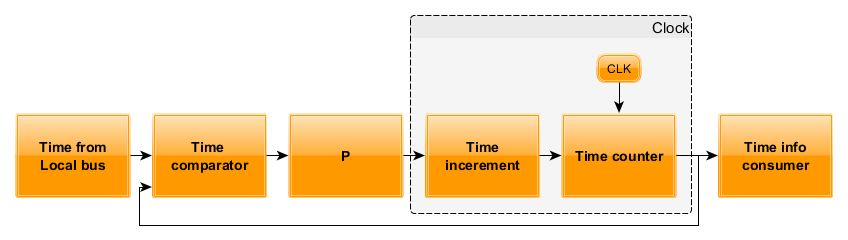
\includegraphics[width=0.7\textwidth]{figures_raw/time_control_loop.png}
    \caption{Internal clock module diagram}
    \label{fig:closed-loop}
\end{figure*}

The frame format used on the bus is shown in Figure~\ref{fig:HiSTI-frame}. The frame starts with an all 1's preamble, and it is
followed by a start bit with value 0. The type field is used to differentiate the payload types. When T=1 it
indicates that the payload is
time information otherwise it is data -- hence an overlay data communication protocol can be used on this data channel.
The time format is in line with the external time synchronization, i.e., it uses the NTP
time format for representing the time information. For detecting transmission errors on the bus, a CRC-8 value is
calculated
for the \emph{`Type'} and \emph{`Payload'} fields and appended to the frame that is checked on frame reception for
detecting
transmission errors.

\begin{equation}\label{eq:tframe}
T_{frame} = N_{bits} \times T_{bit}
\end{equation}
and
\begin{equation}\label{eq:tbit}
T_{bit} = 1/f_{signalling}
\end{equation}

Where T\textsubscript{bit} is the bit time, f\textsubscript{signalling} is the signalling frequency on the internal bus, and N\textsubscript{bits} is the number of bits in the frame.
Calculating \eqref{eq:tframe} and \eqref{eq:tbit} with the above given parameters, the frame time is 90/\SI{15.625}{\mega\hertz} = \SI{5.76}{\micro\second}. Since every
other frame carries time information, the clock on the receiver side can be disciplined/controlled on a
\SI{11.52}{\micro\second}
basis. Under such short period of time even low quality, non-temperature controlled crystal oscillators have negligible
drift.
As a result, this update period is adequate for the network monitoring use case.

The receiver module (i.e., in the FPGA-based Clock Card in Figure~\ref{fig:TymeSinchArch}) de-multiplexes the data and the time information from the payload of the received frame. 
It also verifies that the received frame's CRC-8 value matches the calculated one. If no errors were detected then it feeds the
time information into a module that performs time synchronization executing the pseudo-code in algorithm~\ref{alg:clockdisc}

\begin{algorithm} % enter the algorithm environment
\caption{Receiver local time disciple algorithm} % give the algorithm a caption
\label{alg:clockdisc} % and a label for \ref{} commands later in the document
\begin{algorithmic} % enter the algorithmic environment
    \STATE $Increment \Leftarrow 1/f_{clk}$
    \STATE $Delay_{static} \Leftarrow x$ 
    \STATE $T_{local} \Leftarrow 0$
    \FOR{Each rising edge of system clock}
        \IF{Received valid timestamp from Master}
            \STATE $T_{local} \Leftarrow T_{recv} + Increment + Delay_{static}$
        \ELSE
            \STATE $T_{local} \Leftarrow T_{local} + Increment$
        \ENDIF
    \ENDFOR
\end{algorithmic}
\end{algorithm}

The client clock module -- as shown in Figure~\ref{fig:closed-loop} --
is incrementing a clock counter with an increment value -- corresponding to the nominal clock frequency in the internal time representation -- in each system clock period. The clock module frequency can be adjusted through modifying the time increment itself.
The $Delay_{static}$ constant can be measured for a given configuration and adjusted accordingly. The algorithm is illustrated by a sample waveform of the master and slave entity  in Figure~\ref{fig:internalbus}. Informally if the skew is less than the desired precision under one synchronization period -- i.e. when the valid time is transmitted by the master entity -- then the phase of time progresses in sync on the two entities.

\begin{figure}[!htb]
    \centering
    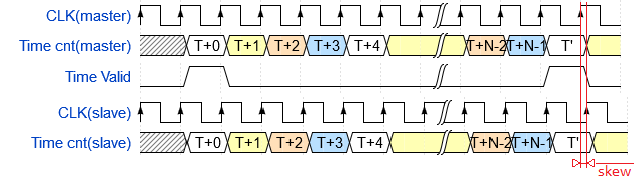
\includegraphics[width=0.5\textwidth]{figures_raw/internalbustiming.png}
    \caption{Illustration of timing on the internal synchronization bus}
    \label{fig:internalbus}
\end{figure}

To concede that this system can have nanosecond synchronization let us execute the algorithm: let $T_n$ be the n\textsuperscript{th} time point where synchronization occurs between the master and the slave entity. At time point $T_n$ when the client receives a timestamp the local clock will be in sync with
the master clock -- given that the $Delay_{static}$ constant was determined correctly. De-synchronization arises due to errors in the master and client clock oscillator frequency. 
To ensure that the desired level of synchronization is reached it has to be shown that the master and client clock would not diverge more than one nanoseconds 
under time interval $(T_n,T_{n+1})$  -- since by definition at $T_{n+1}$ the clocks will be in sync again and this process is periodic. Given a worst case calculation the
following equation must hold true:
\begin{equation}\label{eq:synch}
\begin{aligned} 
\bigg\lvert \frac{1}{(1+\epsilon)f_{clk}}N - \frac{1}{(1-\epsilon)f_{clk}}N  \bigg\rvert  \lesssim 1 ns \\
\frac{N}{f_{clk}} \bigg\lvert \frac{-2\epsilon}{1 - \epsilon ^2} \bigg\rvert \lesssim 1 ns \\
T_{ts} \bigg\lvert \frac{-2\epsilon}{1 - \epsilon ^2} \bigg\rvert \lesssim 1 ns , where \\
N = \frac{T_{ts}}{T_{clk}}
\end{aligned}
\end{equation}

In equation~\ref{eq:synch} $\epsilon$ stands for the precision of the oscillator, $f_{clk}$  is the system clock frequency and $T_{ts}$ is the timestamp frame time on the internal synchronization bus. In theory equation~\ref{eq:synch} can be satisfied for arbitrary $\epsilon$ if $T_{ts}$ can be adjusted freely. Substituting parameters from the concrete implementation with $T_{ts} = 2T_{frame}$ = \SI{11.52}{\micro\second} and $\epsilon$ = 50 ppm results in $1.15 ns \lesssim 1 ns$ which is approximately satisfying. From a practical point of view doubling the clock frequency would have been a small gain in accuracy marginally.


It is important to note that this accuracy and precision is only achieved over the \emph{internal} time synchronization bus. If the external subsystem -- that is completely orthogonal to the internal subsystem -- synchronizes to its reference with \SI{}{\micro\second} accuracy then this results in the same accuracy for the monitoring probe vs. external reference relation. Even though the synchronicity will be still at the \SI{}{\nano\second} level in the monitoring probe vs. monitoring probe relation inside the same monitoring node driven by the same master.

\subsection{Implementation}

The realized system with all internal components is shown by Figure~\ref{fig:realized-system}, where the external time
synchronization -- as presented in Section~\ref{sec:External-Impl} -- is done by the SGA Clock card -- visible in the
bottom right part. Similarly, the internal time synchronization -- described in Section~\ref{sec:Internal-Impl} --
is performed over the local bus with agent modules. These modules run in all the FPGA-based monitoring cards acting as slaves at the
high-speed timestamp interfaces; all are driven by the SGA Clock card acting as a master.

\begin{figure}[H]
    \centering
    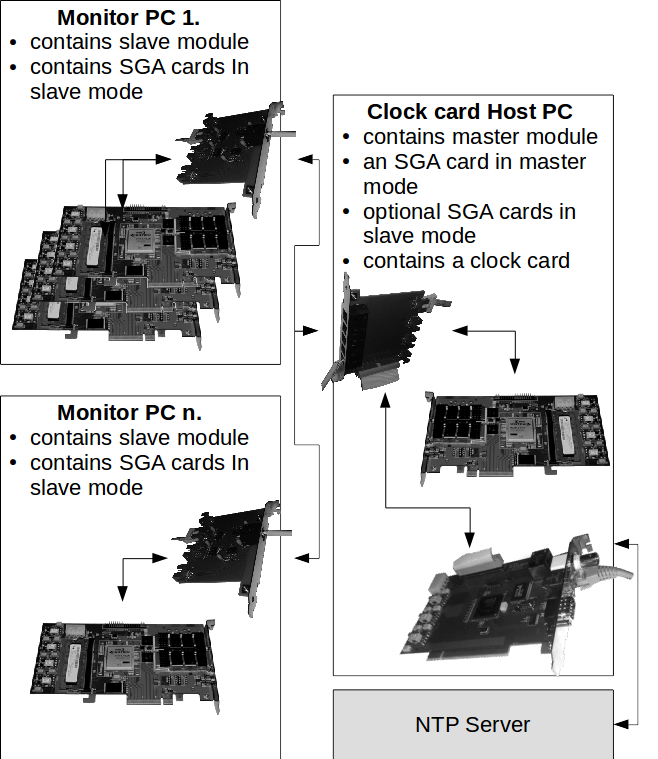
\includegraphics[width=0.45\textwidth]{figures_raw/clock_architecture.png}
    \caption{The realized system with all internal components}
    \label{fig:realized-system}
\end{figure}

\begin{figure*}[!htb]
    \centering
    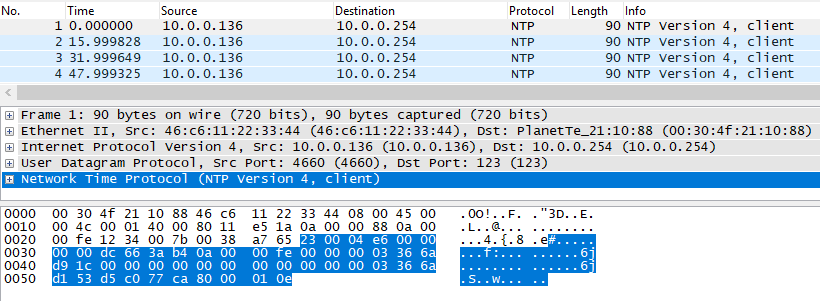
\includegraphics[width=0.9\textwidth]{figures_raw/pcap-NTP.png}
    \caption{Measurement result -- a typical example of an NTP packet containing four timestamps}
    \label{fig:pcap-NTP}
\end{figure*}

\section{Verification \& Results}

%TODO(Fec) : 1.5 oldal
%- Describe the verification method in detail
%- Matlab graph, long-term vs. short-term 

There has been extensive testing and measurements carried out for verifying the solution. In order to analyze the degree of
synchronization to the master NTP clock, a packet capturer was installed on the Ethernet
segment at which the FPGA implementation of the NTP slave was connected. The NTP packets used for synchronization were
captured bidirectionally. This packet capture then was filtered for those NTP packets that had all 4 timestamps used in
the On-Wire protocol to calculate the offset from the reference clock value. Our  dedicated post-processing utility then extracted the
offset information along with the time elapsed from the start of measurement -- which is determined by
the
first NTP packet present in the packet capture.

A sample packet capture is shown by Figure~\ref{fig:pcap-NTP}. The statistical parameters -- like the clock drift and real
offset -- of the device was determined by
fitting a linear curve on the offset values. There were various measurements carried out -- for the actual measurement presented in this paper, the capture was taken
for approximately 3 hours.
The results and the fitted curve plot can be seen on Figure~\ref{fig:results}.

\begin{figure*}[!htb]
    \centering
    \includegraphics[width=0.9\textwidth]{figures_raw/plot2.png}
    \caption{Measurement result -- plot of derived offset-measurement data}
    \label{fig:results}
\end{figure*}

The curve fitted on this measurement shows that there was a fix \SI{14.52}{\micro\second} offset compared to the
reference clock. As presented in Section~\ref{sec:Challanges}
having a precise and stable clock -- with known offset -- is as good as having an accurate one. Besides,
the first order stability of the
device is \SI{-0.7}{1/\nano\second}. This precision and stability are considered adequate for satisfying the
requirements of the external time synchronization part.

As for the internal synchronization part, it is by design accurate as it is a message synchronous bus system with no
disturbances -- even under real-life (but normal) operating conditions. As a
consequence, the clock accuracy over that bus is determined by the bit width (in time duration) and the refresh rate of the digital
time-stamp transmitted over the bus.(See details in Section~\ref{sec:Internal-Impl})
%The proof for that error of the oscillators can be neglected under the refresh time period can be deduced from 
%calculating the skew of the clock periods under a timestamp update period: 

%\begin{equation}\label{eq:clkerr}
%CLK_{skew} = \lfloor  \lvert \frac{2 \times T_{frame}}{T_{sys}} \times E_{oscillator} \rvert \rfloor
%\end{equation}
%
%\begin{equation}
% T_{sys} = 1/f_{sys}
%\end{equation}

%Where T\textsubscript{frame} (frame time over the internal synchornization bus) is \SI{5.76}{\micro\second}, and the typical values of the system clock parameters are
%f\textsubscript{sys} (system clock frequency) is \SI{125}{\mega\hertz} and E\textsubscript{oscillator} (relative frequency error) is $\pm$ 50 ppm.
%Substituting these values into \eqref{eq:clkerr} gives that the skew in terms of clock cycles is $\lfloor 0.072 \rfloor = 0$ clock periods. This is the expected behavior of the %high-precision hardware-based time synchronization for monitoring systems.

%Based on the considerations above, the accuracy simply equals to the resolution of the digital timestamp given by \eqref{eq:resolution}.
%\begin{equation}\label{eq:resolution}
%Resolution = 2^{-N/2} \SI{}{\second}
%\end{equation}

As it was described in Section~\ref{sec:Internal-Impl}, the
timestamp is 64 bits wide -- since it uses the NTP binary fractional representation. 
%with N=64, the theoretical accuracy is \SI{232.83}{\pico\second}. 
The $\sim$\SI{1}{\nano\second} accuracy over the internal synchronization bus satisfies the criteria of any monitoring system with 1, 10 or even 100 Gbit/s Ethernet, since packet interarrival time even of the latter case is 6.72ns \cite{6ns_interarrival} -- almost one magnitude greater than the theoretical accuracy of the presented, implemented and verified time synchronization method.

As a real-life verification, the above described time-synchronization system has been put into operation at Magyar Telekom. The system hardware (with its FPGA firmware) has been installed beside the SGA-7N network monitoring system, and showed the expected result. The system provides accurate time information to the monitoring cards ever since, and it is planned to be expanded for covering all related monitoring cards, network-wide.

\section{Conclusion}

In this paper, we introduced a general time synchronization solution for a high performance, lossless network monitoring system called SGA-7N that is based on a reconfigurable architecture. The probes of the system are called ``Monitors'', which consists of three main building blocks: a high performance Field Programmable Gate Array (FPGA)-based custom hardware platform, a firmware dedicated for network monitoring, and the probe software. The reconfigurable property of the FPGA chip enables to turn the Monitor hardware platform into a high performance networking device -- among others, a network monitoring probe. Beside supporting distributed and lossless packet level monitoring of Ethernet links for 1 or 10 Gbit\/s of the described system, the FPGA serves as the base platform of the time synchronization solution for the interface cards of the Monitors.

Time synchronization of the network monitoring nodes are crucial, since the analysis depends highly on the proper message sequence, which is determined mainly by the timestamps. Using GPS, or PTPv2 in all nodes is not feasible for various reasons, hence this paper proposes a hybrid approach, implemented by utilizing the deterministic processing time of FPGAs.

First, each monitoring site has to have a reference clock that is synchronized with other reference clocks at other sites. Naturally, the monitoring system has to be synchronized to the reference clock available at the physical site. In this paper we call it external time synchronization, and it is solved by an FPGA-based, NTP implementation that use data filtering and has a clock discipline module in order to output monotonous clock information. This avoids timestamps jumping backwards, or jumping forward too much within one step, hence the clock if the monitoring system becomes well-regulated. Each interface at the monitoring node has to get synchronized with this clock information. In this paper we call it internal time synchronization, and it is implemented through a proprietary, rapid protocol. Its sender, (or master) part works in a distributor-card residing at the main reference clock machine of the monitoring system, whereas the receiver (or slave) parts are realized within the FPGA of the monitoring cards.

As presented in the paper, the overall system shows sub-nanosecond accuracy and stability, meeting the requirements of 10 Gbit\/s, or even 100 Gbit\/s Ethernet-based packet monitoring. The presented solution is already installed in the network-wide, real-life monitoring at Magyar Telekom.

\bibliographystyle{IEEEtran}
\bibliography{references}


\begin{IEEEbiography}[{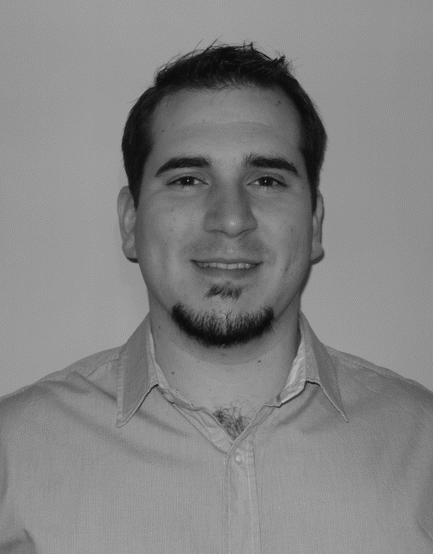
\includegraphics[width=1in,height=1.25in,clip,keepaspectratio]{figures_raw/fj_profile.png}}]{Ferenc Nandor Janky} 
received the MSc degree in Electrical Engineering from BME, Budapest, Hungary, in 2013.
He gained experienced while working for various telecommunication companies including Vodafone, AITIA International Inc. and Ericsson.
His main areas of interest are network protocols, FPGA programming and software development. 
Ferenc is currently working as a C++ software developer for an international corporate bank. He is a member of the SmartComLab at BME TMIT.
\end{IEEEbiography}


\begin{IEEEbiography}[{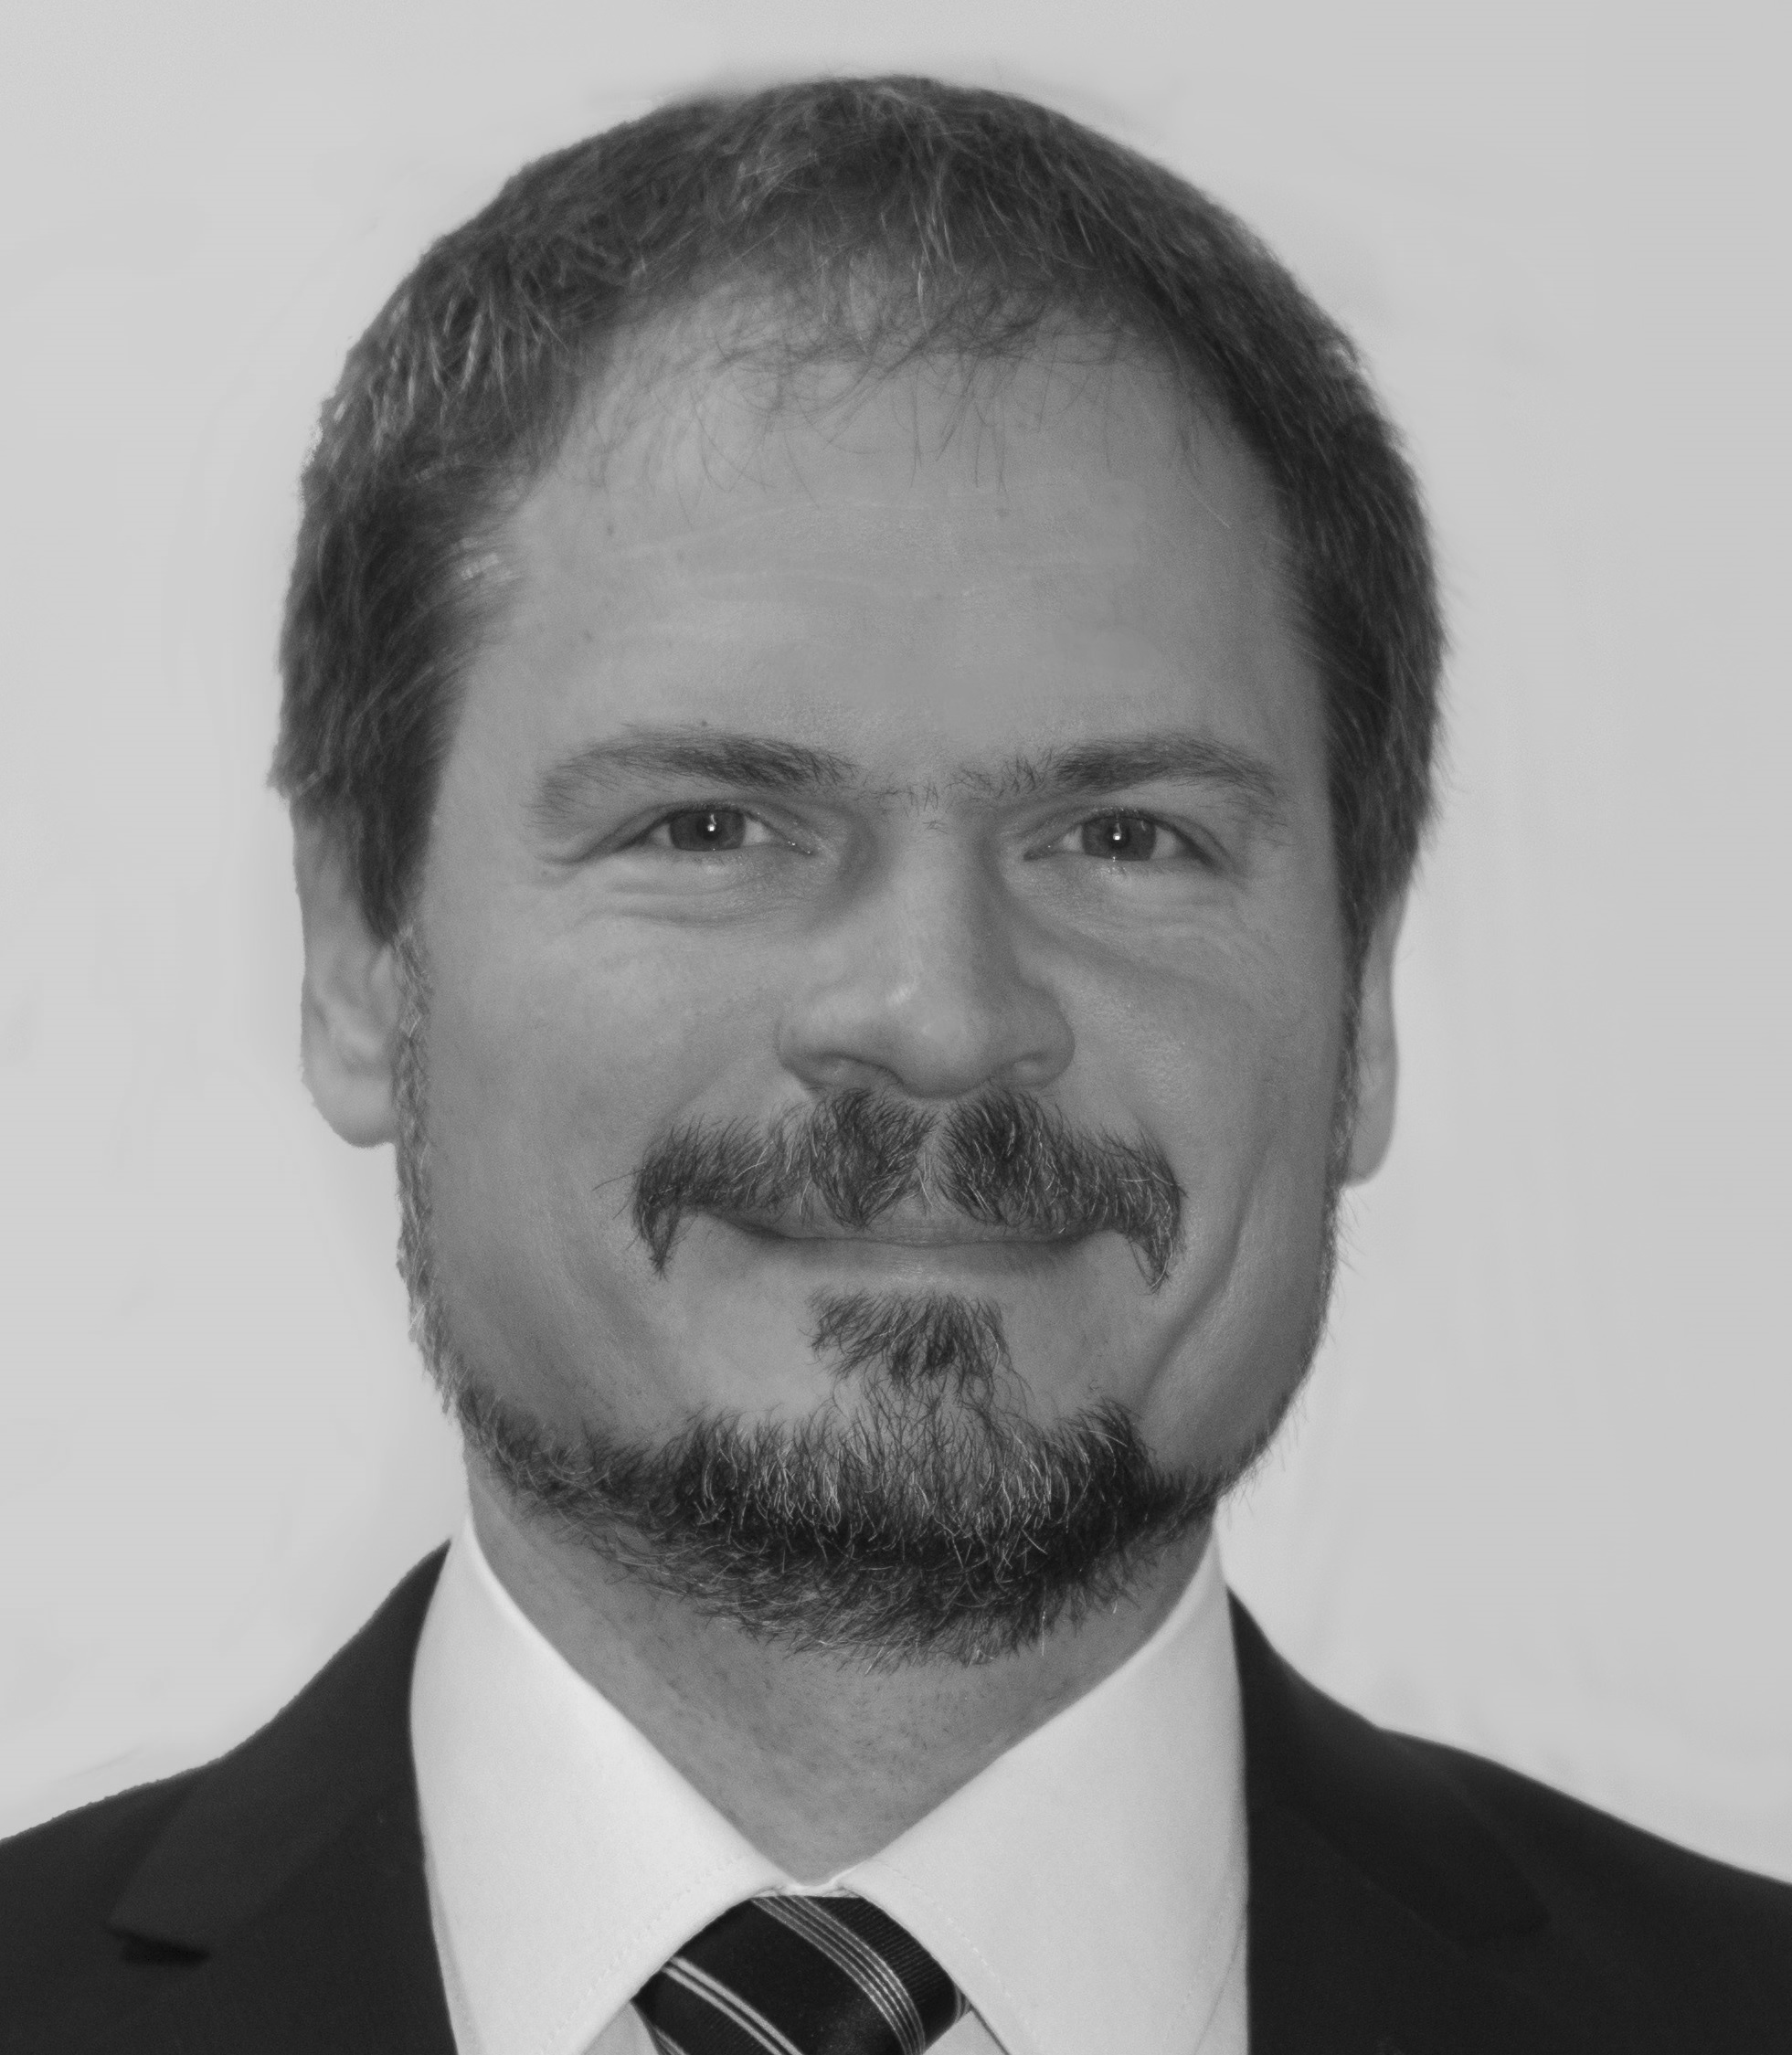
\includegraphics[width=1in,height=1.25in,clip,keepaspectratio]{figures_raw/VP_profile.jpg}}]{Pal Varga}
 is Associate Professor at BME, Hungary, where he received his Ph.D. (2011) from. Besides, he is director in AITIA International Inc. Earlier he was working for Ericsson Hungary and Tecnomen Ireland, as software design engineer and system architect, respectively. His main research interest include network performance measurements, root cause analysis, fault localization, traffic classification, end-to-end QoS and SLA issues, as well as hardware acceleration, and Internet of Things. He is also a member of the SmartComLab at BME TMIT.
% He has been involved in various industrial as well as European research and development projects in these topics.

\end{IEEEbiography}



% http://www.ctan.org/tex-archive/biblio/bibtex/contrib/doc/
% The IEEEtran BibTeX style support page is at:
% http://www.michaelshell.org/tex/ieeetran/bibtex/

%\bibliographystyle{IEEEtran}
% argument is your BibTeX string definitions and bibliography database(s)
%\bibliography{references}

%
% <OR> manually copy in the resultant .bbl file
% set second argument of \begin to the number of references
% (used to reserve space for the reference number labels box)

%\begin{thebibliography}{1}
%
%\bibitem{IEEEhowto:kopka}
%H.~Kopka and P.~W. Daly, \emph{A Guide to \LaTeX}, 3rd~ed.\hskip 1em plus
% 0.5em minus 0.4em\relax Harlow, England: Addison-Wesley, 1999.
%
% \end{thebibliography}

\end{document}
